As previously mentioned (section \ref{sec:chromatin}), epigenetic marks are a fundamental aspect of the cellular biological processes. 
Indeed, their state influences not only gene accession but also the regulation of gene expression.

Some relevant aspects are \glspl{hm} and \glspl{tf}, the first ones are related to transcriptional activation/inactivation, chromosome packaging, and \gls{dna} damaging/repairing, the second ones (\glspl{tf}), also named as sequence-specific \gls{dna}-binding factor, are proteins that control the transcription of genetic information by binding specific sequences of \gls{dna}.

To investigate these epigenetic aspects, the mostly used sequncing technology is the Chromatin ImmunoPrecipitation sequencing (\gls{chipseq}) \cite{Park2009}.
This technique allows to use antibodies for selected proteins or nucleosomes, which enriches for specific \gls{dna} sequences bounded to these proteins/nucleosomes.

\begin{figure}[H]
\centering
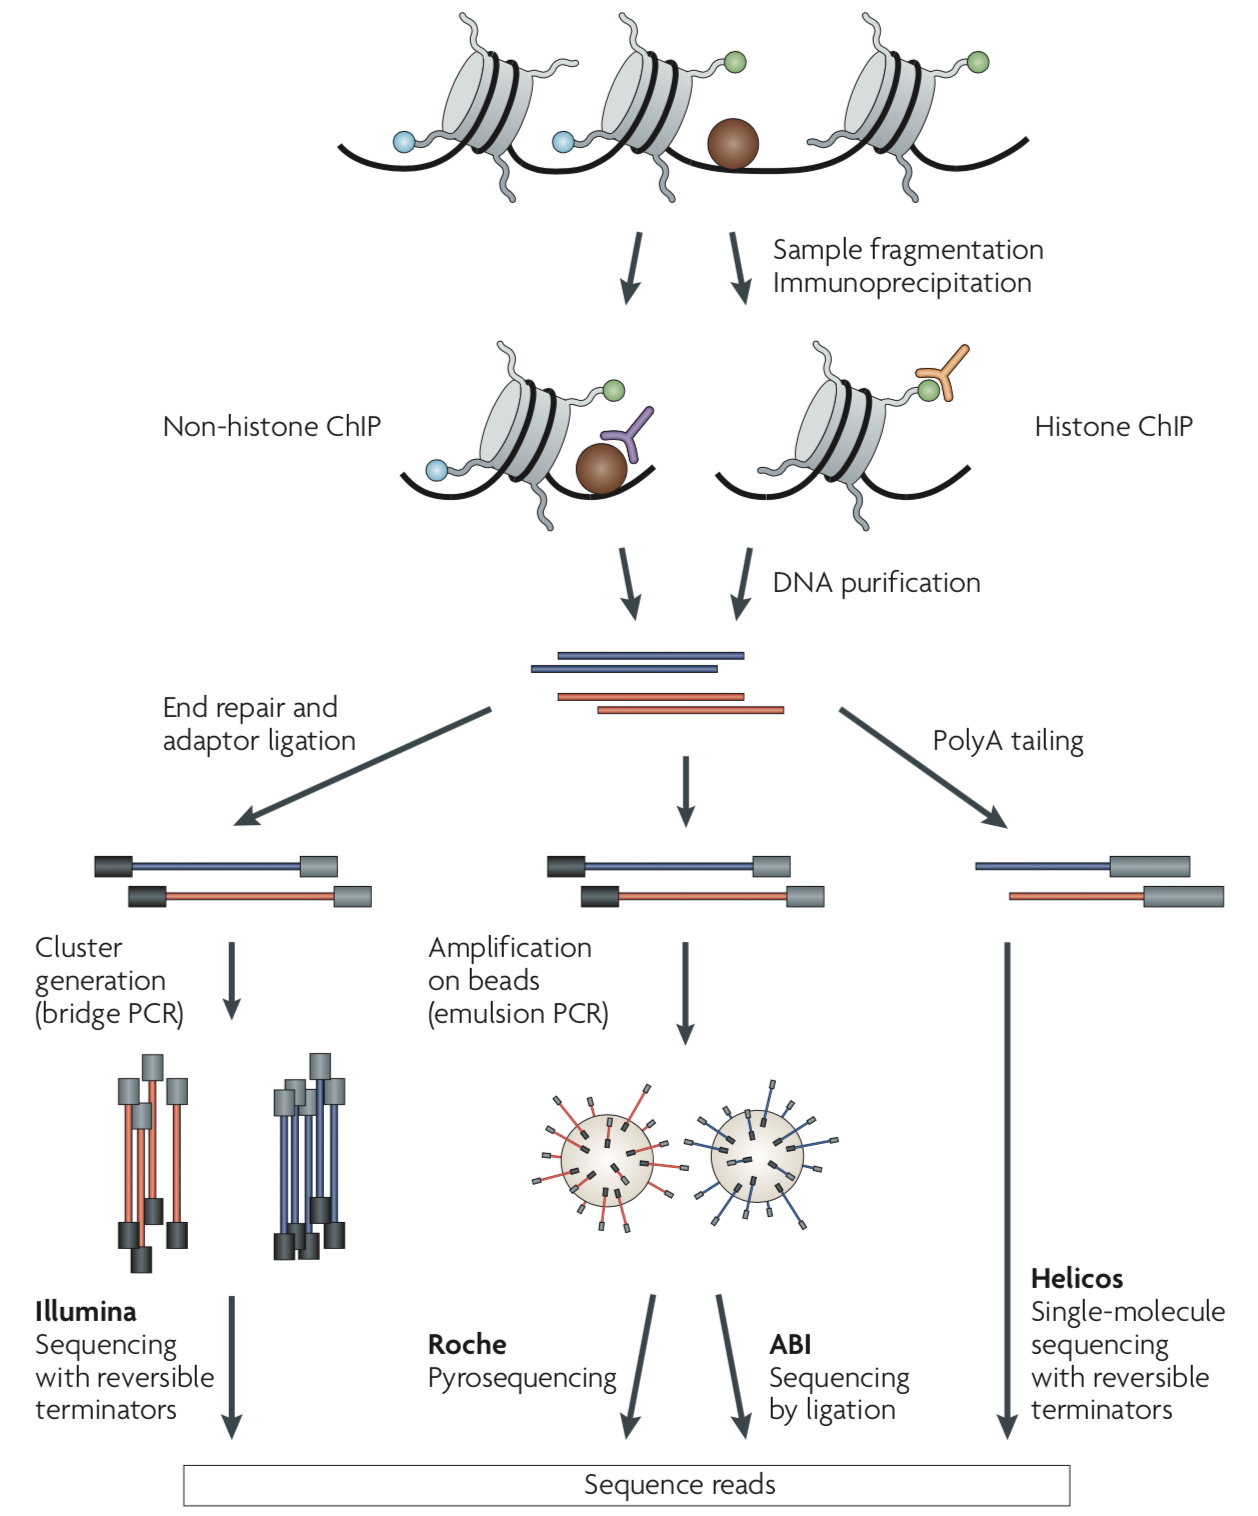
\includegraphics[width=8cm, keepaspectratio]{img/intro/chip.png}
\caption[\gls{chipseq} experiment]{\gls{chipseq} experiments can be used to investigate \gls{dna} binding sites such histone modifications (Histon ChIP) and transcription factors (Non-histone ChIP), using specific antibodies for the specific interested protein (immunoprecipitation).
After the \gls{dna} purification, the genetic matherial is linked to specific adaptors and then amplified in different manner, depending on the amplification and sequencing type used. \cite{Park2009}}
\label{fig:chipseqexp}
\end{figure}

The library preparation consists into locking biological processes with formaldehyde and then cutting the chromatin into small fragments with sonication.
Afterwards, a specific antibody for the interested protein is used to immunoprecipitate the \gls{dna}-protein complex, in order to be purified and, after amplification, to be sequenced.

When analyzing the data, it is relevant to distinguish between \gls{hm} and \gls{tf} ChIP experiments because, even if the library preparation is the same (it differs only for the antibody used, just because the proteins are different), the data analysis pipeline is different on used methodologies because of different signal produced by them.
Indeed, after read mapping on a reference genome, the reads need to be processed with methodologies for the protein-binding regions detection, that are typically called \textit{Peak Callers}.
After the peak calling process it is possible to highlight that the \gls{tf} signals (peaks) are more narrowed respect to the ones detected for \gls{hm}, leading to develop different methodologies for investigating further aspects for each one of these \gls{chipseq} signals.

\begin{figure}[H]
\centering
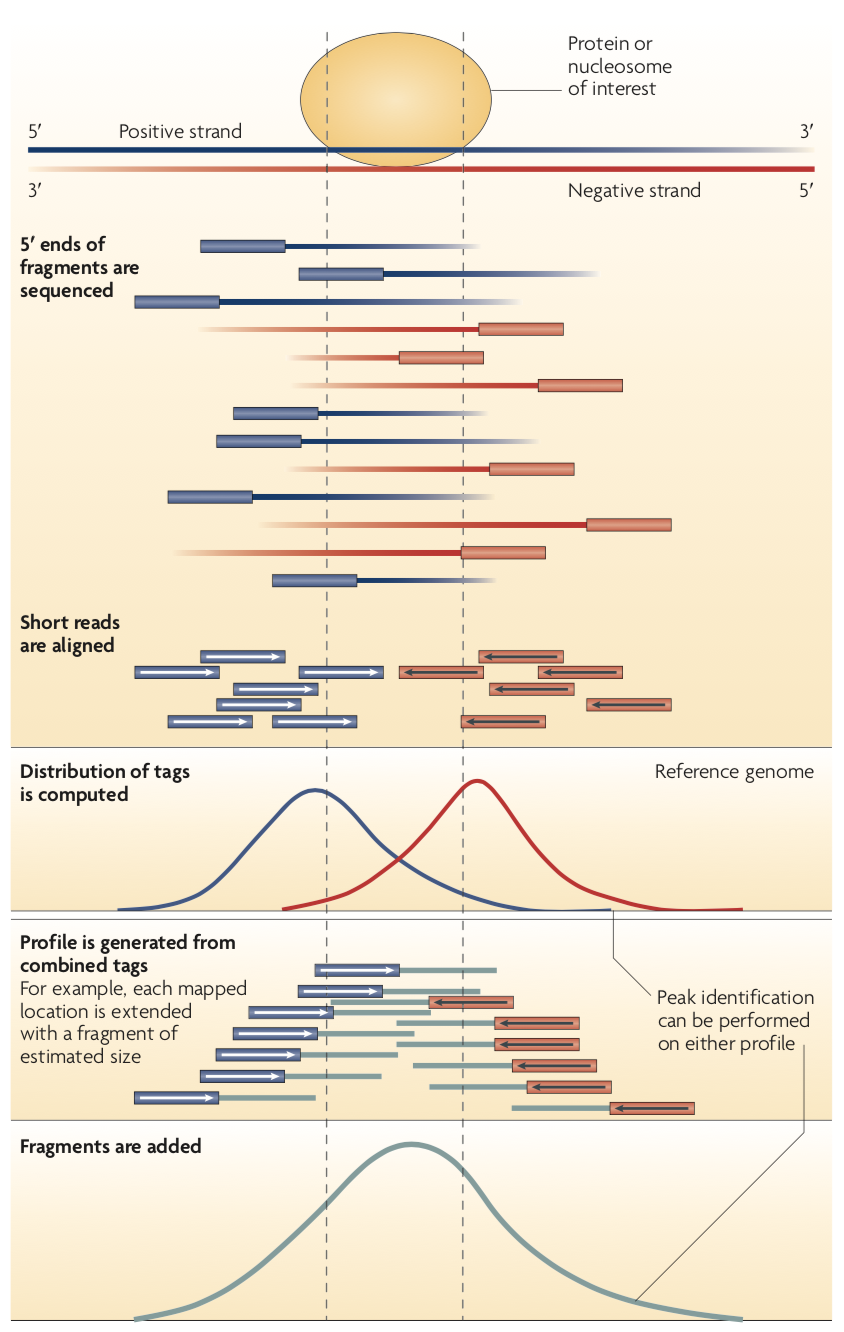
\includegraphics[width=8cm, keepaspectratio]{img/intro/peak_call.png}
\caption[\gls{chipseq} peak detection]{The \gls{dna} fragments at 5' are sequenced, producing a double profile for each \gls{dna} strand in correspondence of the surrounding area of the protein binding site.
In such a way it is possible to identificate a unified peak combining the profiles with the reads.\cite{Park2009}}
\label{fig:chipseqexp}
\end{figure}

Subsequently, after the peak detection, several aspects can be investigated about the signal, such as the identification of peaks related motifs, or the associated genes with detected regions, and, when other omics are available (e.g. \gls{rnaseq}), it is interesting to associate the expressed features (e.g. genes) and doing functional enrichment analysis.





